We know that equation of the line passing through given a point a and in a parallel to $\vec{b}$ is given by
\begin{equation}\label{eq:solutions/line_plane/69/2}
    \vec{r} = \vec{a}+\lambda\vec{b}
\end{equation}
Also we can find direction vector from the Cartesian form of equation
\begin{equation}
    \frac{x-x_1}{a} = \frac{y-y_1}{b} = \frac{z-z_1}{c}
\end{equation}
This can be expressed as
\begin{equation}
    \myvec{x\\y\\z} = \myvec{x_1\\y_1\\z_1} + \lambda\myvec{a\\b\\c}
\end{equation}
where $\vec{a} = \myvec{x_1\\y_1\\z_1}$ is a point on given line and $\vec{b} = \myvec{a\\b\\c}$ is the direction vector.
Writing given equation \eqref{eq:solutions/line_plane/69/1} in vector form as
\begin{equation}
    \myvec{x\\y\\z} = \myvec{3\\-4\\8} + \lambda\myvec{3\\5\\6}
\end{equation}
So the direction vector of equation given is
\begin{equation}\label{eq:solutions/line_plane/69/3}
    \vec{b} = \myvec{3\\5\\6}
\end{equation}
and the point on which line passes is 
\begin{equation}\label{eq:solutions/line_plane/69/4}
   \vec{P} = \myvec{-2\\4\\5} 
\end{equation}
Substituting \eqref{eq:solutions/line_plane/69/3} and \eqref{eq:solutions/line_plane/69/4} in \eqref{eq:solutions/line_plane/69/2} we get
\begin{equation}
    \vec{r} = \myvec{-2\\4\\5} + \lambda \myvec{3\\5\\6}
\end{equation}
which is the line parallel to line \eqref{eq:solutions/line_plane/69/1} and passes through point \myvec{-2\\4\\5}.
\begin{figure}[h]
    \centering
    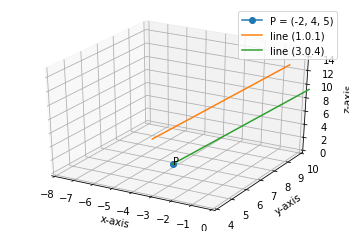
\includegraphics[width=\columnwidth]{./solutions/line_plane/69/fig/figure.png}
    \caption{Equation of line passing through point $P$ and parallel to line \eqref{eq:solutions/line_plane/69/1}}
    \label{fig:}
\end{figure}

